\chapter{Árvores Geradoras Mínimas}

Uma \textbf{árvore geradora} (\emph{spanning tree}) de um grafo conexo e não-direcionado $G = (V, E)$ é um subgrafo que contém todos os vértices de $G$, é conexo e não possui ciclos. 
Em outras palavras, uma árvore geradora conecta todos os vértices de $G$ utilizando exatamente $|V|-1$ arestas.

Dado que um grafo pode possuir diversas árvores geradoras distintas, surge naturalmente o problema de selecionar, entre todas elas, aquela cujo \emph{custo total} seja mínimo. 
Para isso, supõe-se que cada aresta $(u, v)$ de $G$ possui um \emph{peso} $w(u, v)$ associado, representando, por exemplo, a distância, o custo ou o tempo de ligação entre os vértices $u$ e $v$.

Uma \textbf{árvore geradora mínima} (\emph{Minimal Spanning Tree} ou \emph{MST}) é, portanto, uma árvore geradora $T \subseteq G$ que minimiza a soma dos pesos de suas arestas:
\[
w(T) = \sum_{(u,v) \in T} w(u,v)
\]
de modo que $w(T)$ seja o menor possível entre todas as árvores geradoras de $G$.

\subsection*{Aplicações}

O problema da árvore geradora mínima aparece em diversas situações práticas, como:
\begin{itemize}
    \item \textbf{Redes de comunicação:} conectar computadores, roteadores ou cidades com o menor custo possível de cabeamento.
    \item \textbf{Circuitos elétricos:} minimizar o uso de material condutor em uma malha de conexões.
    \item \textbf{Transporte e logística:} planejar estradas, oleodutos ou rotas que conectem pontos de interesse com menor custo total.
    \item \textbf{Agrupamento (clustering):} em aprendizado de máquina, as MSTs podem ser usadas para identificar grupos em conjuntos de dados, eliminando as arestas mais longas.
\end{itemize}

\subsection*{Unicidade da MST}

Em geral, um grafo pode possuir mais de uma árvore geradora mínima, especialmente quando existem arestas com pesos iguais. No entanto, se todos os pesos das arestas forem distintos, então a MST é \textbf{única}. 

Essa propriedade decorre do fato de que, com pesos distintos, qualquer escolha de aresta mínima que respeite as condições de conectividade e ausência de ciclos é forçada -- ou seja, não há empates na decisão de quais arestas pertencem à MST.


\section{Teorema do Corte}

Para compreender os algoritmos de Kruskal e Prim, é essencial entender a propriedade que fundamenta sua correção: o \textbf{Teorema do Corte}. Esse teorema fornece uma condição segura para decidir quando uma aresta pode ser incluída em uma árvore geradora mínima.

\subsection*{Enunciado e Intuição}

Considere um grafo conexo e ponderado $G = (V, E)$ e um \emph{corte} $(S, V - S)$, isto é, uma partição do conjunto de vértices $V$ em dois subconjuntos disjuntos $S$ e $V - S$.

Dizemos que uma aresta \emph{cruza o corte} se ela tem uma extremidade em $S$ e outra em $V - S$. 
Um corte é dito \emph{seguro} para uma árvore parcial $T$ se nenhuma das arestas de $T$ cruza o corte — ou seja, se $T$ está contido inteiramente em um dos lados da partição.

\begin{theorem}[Teorema do Corte]
Seja $(S, V - S)$ um corte em $G$ que respeita uma árvore parcial $T$ (isto é, nenhuma aresta de $T$ cruza o corte). 
Então, a aresta de menor peso que cruza esse corte é \textbf{segura}, ou seja, pertence a \emph{alguma} árvore geradora mínima de $G$.
\end{theorem}

A intuição é simples: se dividirmos o grafo em dois grupos de vértices, a melhor maneira de conectá-los sem criar ciclos é escolhendo a aresta mais leve que liga esses dois grupos. 
Qualquer outra escolha aumentaria o custo total da árvore.

\subsection*{Demonstração Intuitiva}

Suponha que a aresta $(u, v)$ seja a de menor peso que cruza o corte $(S, V - S)$, e que $T^*$ seja uma árvore geradora mínima que não contém $(u, v)$.

Como $T^*$ é uma árvore, há exatamente um caminho entre $u$ e $v$ em $T^*$. 
Esse caminho deve cruzar o corte em alguma outra aresta $(x, y)$, que conecta $S$ e $V - S$. 

Como $(u, v)$ é a aresta de menor peso que cruza o corte, temos $w(u, v) \leq w(x, y)$. 
Se substituirmos $(x, y)$ por $(u, v)$ em $T^*$, obtemos uma nova árvore $T'$ cujo peso total não é maior que o de $T^*$. Logo, $T'$ também é uma árvore geradora mínima e contém $(u, v)$. 

Portanto, a aresta de menor peso que cruza um corte seguro sempre pertence a alguma MST.

\subsection*{Importância do Teorema}

O Teorema do Corte é a base teórica que garante a correção dos dois principais algoritmos de obtenção da árvore geradora mínima:

\begin{itemize}
    \item \textbf{Algoritmo de Kruskal:} em cada passo, escolhe a aresta de menor peso que conecta dois componentes distintos da floresta atual (ou seja, cruza um corte seguro). 
    O teorema garante que essa escolha é sempre válida.
    \item \textbf{Algoritmo de Prim:} cresce uma árvore a partir de um vértice inicial, sempre adicionando a aresta de menor peso que liga um vértice fora da árvore a um vértice dentro dela. Essa aresta também cruza um corte seguro.
\end{itemize}

Assim, tanto Kruskal quanto Prim podem ser vistos como aplicações diretas do Teorema do Corte: em cada passo, eles identificam um corte e escolhem a aresta mais leve que o cruza, garantindo que o resultado final será uma árvore geradora mínima.

\subsection*{Exemplo Gráfico}

A Figura~\ref{fig:cut-theorem} ilustra o conceito de corte e a escolha de uma aresta segura.

\begin{figure}[h]
\centering
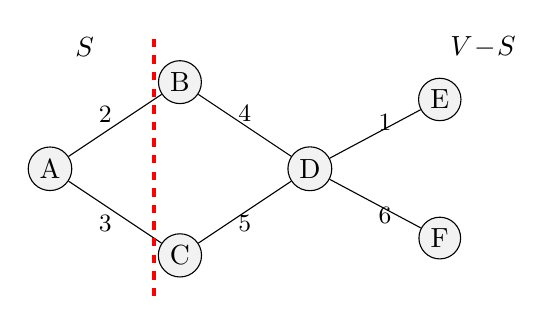
\begin{tikzpicture}[scale=1.1]
% estilos separados
\tikzset{
  vertex/.style={circle, draw, fill=gray!10, inner sep=2pt},
  w/.style={draw=none, fill=none, inner sep=1pt, font=\small}
}

\node[vertex] (a) at (0,0) {A};
\node[vertex] (b) at (1.5,1) {B};
\node[vertex] (c) at (1.5,-1) {C};
\node[vertex] (d) at (3,0) {D};
\node[vertex] (e) at (4.5,0.8) {E};
\node[vertex] (f) at (4.5,-0.8) {F};

\draw (a) -- node[w, above left]{2} (b);
\draw (a) -- node[w, below left]{3} (c);
\draw[dashed, very thick, red] (1.2,1.5) -- (1.2,-1.5);
\draw (b) -- node[w, above]{4} (d);
\draw (c) -- node[w, below]{5} (d);
\draw (d) -- node[w, above right]{1} (e);
\draw (d) -- node[w, below right]{6} (f);

\node[draw=none, fill=none] at (0.4,1.4) {$S$};
\node[draw=none, fill=none] at (5,1.4) {$V\!-\!S$};
\end{tikzpicture}
\caption{A aresta de menor peso que cruza o corte (em vermelho) é segura e pertence a alguma MST.}
\label{fig:cut-theorem}
\end{figure}


\section{Algoritmo de Kruskal}

O algoritmo de Kruskal é uma das abordagens clássicas para encontrar a \textbf{árvore geradora mínima (MST)} de um grafo ponderado. 
Ele segue uma estratégia \emph{gananciosa} (greedy), escolhendo em cada passo a aresta de menor peso que não forme ciclo com as arestas já selecionadas.

\subsection*{Ideia Intuitiva}

A ideia é simples: comece com uma \emph{floresta} (um conjunto de vértices desconectados) e, a cada passo, una dois componentes distintos por meio da aresta de menor peso que os conecta. 
O processo continua até que todos os vértices estejam conectados em uma única árvore.

Esse crescimento por união de componentes justifica a necessidade de uma estrutura eficiente para verificar se dois vértices pertencem ao mesmo componente -- essa é a função da estrutura de dados \textbf{união-busca} (\emph{disjoint-set union}, DSU), também chamada de \emph{union–find}.

\subsection*{Estrutura de Dados: União-Busca}

A estrutura de união-busca mantém uma partição dos vértices em conjuntos disjuntos e oferece duas operações básicas:

\begin{itemize}
    \item \texttt{find(u)}: retorna o representante (raiz) do conjunto ao qual o vértice $u$ pertence;
    \item \texttt{union(u, v)}: une os conjuntos que contêm $u$ e $v$, caso sejam distintos.
\end{itemize}

As implementações eficientes de \texttt{union–find} utilizam \textbf{compressão de caminho} e \textbf{união por rank}, garantindo tempo praticamente constante para cada operação: 
$O(\alpha(V))$, onde $\alpha$ é a \emph{função inversa de Ackermann}, que cresce muito lentamente.

\subsection*{Implementação}

A seguir, apresentamos uma implementação simplificada do algoritmo de Kruskal em linguagem C, utilizando a estrutura de dados união-busca.

\begin{lstlisting}[language=C, caption={Implementação do algoritmo de Kruskal utilizando o TAD União–Busca}, label={lst:kruskal-tad}]
#include <stdio.h>
#include <stdlib.h>
#include "union-find.h"   // TAD de conjuntos disjuntos

typedef struct {
    int u, v;
    int peso;
} Aresta;

int compara(const void* a, const void* b) {
    Aresta* A = (Aresta*)a;
    Aresta* B = (Aresta*)b;
    return A->peso - B->peso;
}

void kruskal(Aresta arestas[], int nVertices, int nArestas) {
    UF* uf = uf_criar(nVertices);
    qsort(arestas, nArestas, sizeof(Aresta), compara);

    printf("Arestas da MST:\n");
    int total = 0;

    for (int i = 0; i < nArestas; i++) {
        int u = arestas[i].u;
        int v = arestas[i].v;

        if (uf_find(uf, u) != uf_find(uf, v)) {
            uf_unir(uf, u, v);
            printf("(%d, %d) peso=%d\n", u, v, arestas[i].peso);
            total += arestas[i].peso;
        }
    }

    printf("Custo total da MST = %d\n", total);
    uf_destruir(uf);
}
\end{lstlisting}

\subsection*{Exemplo Passo a Passo}

Considere o grafo a seguir com pesos nas arestas:

\[
A - B (1), \quad B - C (3), \quad A - C (2), \quad C - D (4)
\]

\begin{enumerate}
    \item Ordenamos as arestas por peso: $(A,B)$, $(A,C)$, $(B,C)$, $(C,D)$.
    \item Inicialmente, cada vértice é seu próprio conjunto.
    \item Adicionamos $(A,B)$ $\rightarrow$ une $A$ e $B$.
    \item Adicionamos $(A,C)$ $\rightarrow$ une $(A,B)$ com $C$.
    \item Aresta $(B,C)$ é descartada, pois criaria um ciclo.
    \item Adicionamos $(C,D)$ $\rightarrow$ une $D$ ao conjunto.
\end{enumerate}

Resultado: MST = $\{(A,B), (A,C), (C,D)\}$, custo total = $1 + 2 + 4 = 7$.

\subsection*{Análise de Complexidade}

\begin{itemize}
    \item A ordenação das arestas requer $O(E \log E)$.
    \item Cada operação de união ou busca custa $O(\alpha(V))$, o que é praticamente constante.
    \item Assim, a complexidade total é:
    \[
    O(E \log E + E \alpha(V)) = O(E \log V)
    \]
\end{itemize}

\subsection*{Discussão}

O algoritmo de Kruskal é particularmente eficiente para \textbf{grafos esparsos}, nos quais o número de arestas $E$ é próximo de $V$.  
Por usar uma estrutura baseada em conjuntos disjuntos, é simples de implementar e fácil de adaptar a diferentes representações de grafos (lista de arestas, arquivos, etc.).  
Seu comportamento se degrada apenas em grafos muito densos, onde o custo de ordenar todas as arestas passa a dominar.

\section{Algoritmo de Prim}

O algoritmo de Prim é outra estratégia clássica para encontrar a \textbf{árvore geradora mínima (MST)} em um grafo ponderado e conexo. 
Assim como o algoritmo de Kruskal, ele segue uma abordagem \emph{gananciosa} (greedy), mas adota uma perspectiva diferente: 
em vez de unir componentes desconexos, o algoritmo \textbf{cresce uma única árvore} a partir de um vértice inicial, adicionando sempre a aresta de menor peso que conecta a árvore a um novo vértice.

\subsection*{Ideia Intuitiva}

O algoritmo parte de um vértice arbitrário e constrói a MST de forma incremental. A cada iteração:
\begin{enumerate}
    \item Considera todas as arestas que ligam um vértice já incluído na árvore a um vértice ainda fora dela;
    \item Escolhe a aresta de menor peso entre essas;
    \item Adiciona o novo vértice e a aresta correspondente à árvore.
\end{enumerate}

O processo termina quando todos os vértices foram incluídos. O conjunto das arestas escolhidas forma a árvore geradora mínima.

\subsection*{Estrutura de Dados: Fila de Prioridade}

Para selecionar eficientemente a próxima aresta de menor peso, o algoritmo de Prim utiliza uma \textbf{fila de prioridade mínima} (geralmente implementada como um \emph{heap binário}).  

Cada vértice $v$ mantém um valor \texttt{chave[v]}, que representa o menor peso de uma aresta que conecta $v$ a algum vértice já pertencente à árvore.  
A fila de prioridade permite extrair o vértice de menor \texttt{chave} em $O(\log V)$ e atualizar o valor das chaves de seus vizinhos em $O(\log V)$.

\subsection*{Implementação}

Abaixo está uma versão simplificada do algoritmo de Prim em C, utilizando uma representação de grafo por matriz de adjacência e uma fila de prioridade implementada com busca linear (para clareza didática).

\begin{lstlisting}[language=C, caption={Implementação do algoritmo de Prim em C}, label={lst:prim}]
#include <stdio.h>
#include <limits.h>
#include <stdbool.h>

#define V 5 // número máximo de vértices

int menorChave(int chave[], bool incluido[]) {
    int min = INT_MAX, min_index;
    for (int v = 0; v < V; v++)
        if (!incluido[v] && chave[v] < min)
            min = chave[v], min_index = v;
    return min_index;
}

void prim(int grafo[V][V]) {
    int pai[V];     // para armazenar a MST
    int chave[V];   // menor peso até cada vértice
    bool incluido[V]; // se o vértice já foi incluído

    for (int i = 0; i < V; i++) {
        chave[i] = INT_MAX;
        incluido[i] = false;
    }

    chave[0] = 0;  // começa do vértice 0
    pai[0] = -1;   // raiz da MST

    for (int cont = 0; cont < V - 1; cont++) {
        int u = menorChave(chave, incluido);
        incluido[u] = true;

        for (int v = 0; v < V; v++)
            if (grafo[u][v] && !incluido[v] && grafo[u][v] < chave[v]) {
                pai[v] = u;
                chave[v] = grafo[u][v];
            }
    }

    printf("Arestas da MST:\n");
    int total = 0;
    for (int i = 1; i < V; i++) {
        printf("%d - %d  peso=%d\n", pai[i], i, grafo[i][pai[i]]);
        total += grafo[i][pai[i]];
    }
    printf("Custo total da MST = %d\n", total);
}
\end{lstlisting}

\subsection*{Exemplo Passo a Passo}

Considerando o grafo da Figura~\ref{fig:prim-example}, o algoritmo de Prim parte do vértice $A$ e segue o seguinte processo:

\begin{enumerate}
    \item Começa em $A$, define \texttt{chave[A] = 0}.
	\item Escolhe $(A,B)$ como a aresta mais leve conectando a árvore a um novo vértice.
    \item Escolhe $(B,C)$, depois $(A,D)$, e finalmente $(B,E)$.
\end{enumerate}

Ao final, temos a MST formada pelas arestas $\{(A,B), (B,C), (A,D), (B,E)\}$.

\begin{figure}[h]
\centering
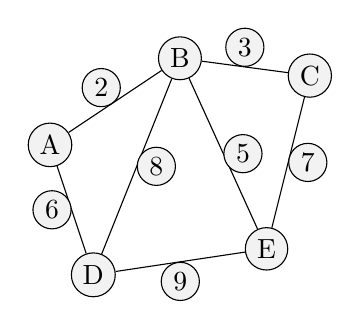
\begin{tikzpicture}[scale=1.1, every node/.style={circle, draw, fill=gray!10, inner sep=2pt}]
\node (a) at (0,0) {A};
\node (b) at (1.5,1) {B};
\node (c) at (3,0.8) {C};
\node (d) at (0.5,-1.5) {D};
\node (e) at (2.5,-1.2) {E};

\draw (a)--node[above left]{2}(b);
\draw (b)--node[above]{3}(c);
\draw (a)--node[left]{6}(d);
\draw (b)--node[right]{8}(d);
\draw (b)--node[right]{5}(e);
\draw (c)--node[right]{7}(e);
\draw (d)--node[below]{9}(e);
\end{tikzpicture}
\caption{Exemplo de grafo usado no algoritmo de Prim.}
\label{fig:prim-example}
\end{figure}

\subsection*{Análise de Complexidade}

A complexidade depende da estrutura usada para a fila de prioridade:

\begin{itemize}
    \item Com \textbf{heap binário}: cada inserção ou atualização custa $O(\log V)$, resultando em $O(E \log V)$.
    \item Com \textbf{heap de Fibonacci}: a operação \texttt{decrease\_key} é $O(1)$ amortizado, reduzindo a complexidade total para $O(E + V \log V)$.
\end{itemize}

\subsection*{Discussão}

O algoritmo de Prim tende a ser mais eficiente em \textbf{grafos densos}, pois evita a ordenação global de arestas. 
Ele é especialmente adequado para grafos representados por \textbf{matriz de adjacência}, enquanto o algoritmo de Kruskal é preferível em grafos esparsos representados por \textbf{lista de arestas}.

Ambos os algoritmos são corretos e produzem o mesmo resultado -- mas Prim costuma apresentar melhor desempenho quando o número de arestas é grande em relação ao número de vértices.

\section{Comparação e Discussão}

Os algoritmos de Kruskal e Prim resolvem o mesmo problema -- encontrar a árvore geradora mínima -- e produzem resultados idênticos para qualquer grafo conexo e ponderado. 
No entanto, suas estratégias e estruturas de dados são distintas, o que faz com que cada um apresente vantagens em contextos diferentes.

O algoritmo de \textbf{Kruskal} é baseado na ideia de crescer uma \emph{floresta}, unindo componentes desconexos com a aresta de menor peso que não forma ciclo. 
Já o algoritmo de \textbf{Prim} cresce uma \emph{única árvore}, expandindo-a a partir de um vértice inicial.

A seguir, resumimos as principais diferenças entre os dois métodos:

\begin{table}[h]
\centering
\begin{tabular}{|l|c|c|}
\hline
\textbf{Característica} & \textbf{Kruskal} & \textbf{Prim} \\ \hline
\textbf{Estrutura principal} & União-busca & Fila de prioridade \\ \hline
\textbf{Estratégia} & Cresce floresta & Cresce árvore \\ \hline
\textbf{Complexidade} & $O(E \log V)$ & $O(E \log V)$ \\ \hline
\textbf{Grafos ideais} & Esparsos & Densos \\ \hline
\textbf{Implementação} & Mais simples & Mais eficiente em alguns casos \\ \hline
\end{tabular}
\caption{Comparação entre os algoritmos de Kruskal e Prim.}
\label{tab:kruskal-vs-prim}
\end{table}

Ambos são algoritmos \emph{gananciosos} (\emph{greedy}) e fundamentam-se no \textbf{Teorema do Corte}, que garante que a escolha local da menor aresta que cruza um corte seguro leva a uma solução global ótima.  

Em termos práticos:
\begin{itemize}
    \item Kruskal é preferido quando o grafo é \textbf{esparso} e representado por uma lista de arestas, pois exige apenas a ordenação inicial e operações simples de união-busca.
    \item Prim tende a ser mais eficiente em \textbf{grafos densos} e quando o grafo é representado por uma matriz de adjacência, especialmente se for implementado com um heap.
\end{itemize}

Ambos os métodos ilustram bem a filosofia dos algoritmos gananciosos: construir a solução passo a passo, tomando sempre a decisão local que parece melhor, e ainda assim alcançar o ótimo global.

